% !TEX root = BA-Bericht.tex
\chapter{Ideen und Konzepte}
\label{ch:ideen_und_konzepte}

Dieses Kapitel zeigt Ideen auf, wie die Fragestellung angegangen wurde.
Es wird ein Konzept für einen Teststand vorgestellt, der den Anforderungen (siehe Abschnitt~\fullref{sub:Anforderungen}) gerecht wird.



% TODO Beschreibung wie das Problem im Ansatz gelöst werden soll

% Hier geht es um die Fragestellung, wie Sie die formulierten Ziele der Arbeit erreichen wollen.
% Sie halten z.B. erste, grobe Ideen, skizzenhafte Lösungsansätze fest. Gibt es mehrere Wege, Ansätze
% um dieses Ziel zu erreichen, begründen Sie hier, warum Sie einen bestimmten Weg einschlagen.
% Beispiel für ein Softwareprojekt: Erste Gedanken über eine grobe Systemarchitektur. Ist z.B. eine
% Microservice-Architektur angebracht? Welche Alternativen bestehen, wo gibt es Problempunkte? Die
% Umsetzung, die Beurteilung der Machbarkeit und die detaillierte Beschreibung der umgesetzten
% Architektur sind dann Teil der Realisierung.

% Abgrenzung zu Kapitel 5 (Realisierung):
% - Besteht ein wesentliches Projektziel darin, für Ihre Kunden z.B. ein Security-Konzept, ein
% Kommunikations-Konzeptes, ein IT-Fachkonzept oder ein anderes Fach-Konzept zu erstellen, dann
% wird die Entwicklung dieser (fachlichen) Konzepte unter «Realisierung» beschrieben (sie sind ja der
% eigentliche Kern Ihrer Arbeit).
% - Besteht z.B. ein wesentliches Ziel der Arbeit darin, eine passende Software-Architektur zu
% evaluieren, dann gehören die entsprechenden Beschreibungen ins Kapitel 5.

Grundsätzlich soll ein Teststand aufgebaut werden, an dem empirische Performance Messungen an einem I2P-Testnetzwerk durchgeführt werden können \seereq{TINF}.
Dabei gibt es verschiedene Herausforderungen und Aspekte die es zu beachten gilt.
In den folgenden Abschnitten werden nun Ideen vorgestellt und genauer erläutert, wie diese Herausforderungen angegangen werden.
In den folgenden Abschnitten werden verschiedene Lösungsansätze für verschiedene Teilprobleme und Aspekte vorgestellt.

%TODO: Hyptohesen kann man testen, bestätigen, neue hyptothesen & und oder neue Tests
%TODO: das empirische
%TODO: hat nichts mit I2P

%TODO: 2. isolieres netzwerk
%TODO: 3. technologie ideen / Realisierungsvariianten

\section{Reproduzierbarkeit}

Um Messungen auf einem solchen Testnetzwerk wiederholbar und so gut wie möglich reproduzierbar zu machen \seereq{TREP}, sind folgende zwei Ideen wichtig.
Als erstes soll das Testnetzwerk isoliert werden, um äussere Einflüsse durch das Netzwerk (auch das öffentliche I2P-Netzwerk) zu vermeiden (siehe auch Abschnitt~\ref{sec:isolierung}).
Zweiteres soll die Testinfrastruktur als Programmcode beschrieben werden (auch bekannt als \glstext{iac} (\glsname{iac})).
Somit kann dasselbe Testnetzwerk später wieder erneut wieder aufgebaut werden, anhand der versionierten Infrastrukturdefinition.
Mehr dazu im Abschnitt~\ref{sec:infrastructure}.

\section{Infrastruktur}\label{sec:infrastructure}

Wichtig für das Deployment der Infrastruktur für das Testnetzwerk ist, dass man schnell neue Messungen starten und neue Testnetzwerke erstellen kann \seereq{TPER}.
Dies auch mit der Möglichkeit verschiedene Konfigurationseinstellungen tätigen zu können \seereq{TCNF}.
Die im Vorherigen Abschnitt bereits erwähnt, soll das Deployment auch reproduzierbar sein \seereq{TREP}.
Es soll auch möglich sein verschieden grosse Testnetzwerke zu erstellen \seereq{TSCL}.

\subsection{Container oder Virtuelle Maschinen}

Um Ressourcen zu schonen und aufgrund von kleinerem Overhead sowie Startup-Time von Containern im Gegensatz zu virtuellen Maschinen sind diese wohl zu bevorzugen.
Zudem lassen sich Container schneller neu zu erstellen und zu deployen.
Container erlauben es auch schneller Tests durchzuführen \seereq{TPER}. 
aber auch Tests mit mehr Knoten zu machen, da weniger Ressourcen für einen einzelnen Knoten benötigt wird, da der Betriebssystemkernel geteilt wird.
Dies ist der Fall weil bei Containerlösungen (oder auch OS-Virtualisierung) im Gegensatz zu Virtuellen Maschinen der Betriebssystemkernel zwischen den Instanzen geteilt wird.

\subsection{Deployment}

%TODO: Dies ist eine realisierungsfrage

Es gibt verschiedene Tools für das Deployment von gesamten Netzwerken, virtuellen Maschinen oder Container erlauben. 
Diese sind z.B. Docker-Compose, Kubernetes, Teraform, oder auch NixOps.
Wobei bereits Erfahrungen gemacht wurden mit NixOps und Docker-Compose.
Aufgrund dessen wird eine Lösung diesen Tools angestrebt.
Diese Tools erlauben ein reproduzierbares Deployment.
Dies wird vor allem von NixOps als Feature angepriesen.

\section{Konfigurierbarkeit}

Nach Absprache mit dem Auftraggeber soll mindestens folgendes soll im Teststand konfigurierbar sein (\reqref{TCNF}):

\begin{itemize}
    \item Anzahl-Knoten im Testnetzwerk
    \item Maximale Bandbreite der einzelnen Knoten
    \item Anzahl Hops (Also die Länge der Tunnel)
    \item Ob im privaten oder öffentlichen Netzwerk getestet werden soll. (optional)
\end{itemize}

Nix als deklarative Konfigurationssprache erlaubt es beliebige Aspekte des Setups konfigurierbar zu machen.
Die meisten oben erwähnten Konfigurationsmöglichkeiten werden bereits durch verschiedene NixOS-Module (\lstinline|i2pd|, \lstinline|firewall|, ... ) angeboten.
Als anderer Ansatz kann eine JSON-Datei eingesetzt werden, da diese von vielen Programmiersprachen einfach eingelesen werden können.

\section{Latenzmessung}

Um die Latenz oder Verzögerung einer Nachricht im Testnetzwerks zu messen \seereq{TLAT}, könnte man jeweils den Empfangs- sowie Sendezeitpunkt einer Nachricht speichern und voneinander subtrahieren.

\indexequation{Latenz = Empfangszeitpunkt - Sendezeitpunkt}{Latenzberechnung}{Latenzberechnung}

Jedoch muss sichergestellt werden, dass die Uhrzeiten zwischen allen Knoten synchron ist.
Grundlage für eine saubere Latenzmessung ist zudem, dass man in keine Ressourcenengpässe gerät.
Dementsprechend ist das Überwachen der benötigen Ressourcen wichtig. Siehe dazu Abschnitt~\fullref{sec:ressourcenauslastung}.

\section{Limitieren der Bandbreite}

Die \lstinline|i2pd|-Software erlaubt es die Bandbreite eines Knotens \seereq{TLIM} mittels der \lstinline|bandwidth| Konfigurationseinstellung \seereq{TCNF} zu limitieren. \parencite{noauthor_i2p_nodate-3}
Zusätzlich gäbe es auch andere Wege die Bandbreite zu limitieren.
Eine Möglichkeit wäre dies auf Netzwerkebene mittels dem ``Traffic Control Tool'' (kurz \lstinline|tc| zu lösen.

\section{Isolierung des Testnetzwerks}
\label{sec:isolierung}

% äussere einflüsse / idealisierte umgebung
Um äussere Einflüsse zu vermeiden und eine idealisierte Testumgebung zu erschaffen muss das Testnetzwerk isoliert werden.
Das Diagramm~\fullref{fig:i2p-testnetwork} zeigt den Aufbau des Testnetzwerks auf.
Einerseits kann eine Isolation auf Ressourcenebene durch die verwendete virtuelle Maschine erreicht werden.
Andererseits stellt dies auch automatisch eine Netzwerkisolation zur Verfügung, je nach dem wie die Virtuelle Maschine mit dem Host verbunden wird.
Das Testnetzwerk soll standardmässig weder mit dem Internet verbunden, noch mit dem System des Testers, um äussere Einflüsse zu verringern und somit durch Isolation bessere Reproduzierbarkeit zu erreichen.

\begin{figure*}[ht]
  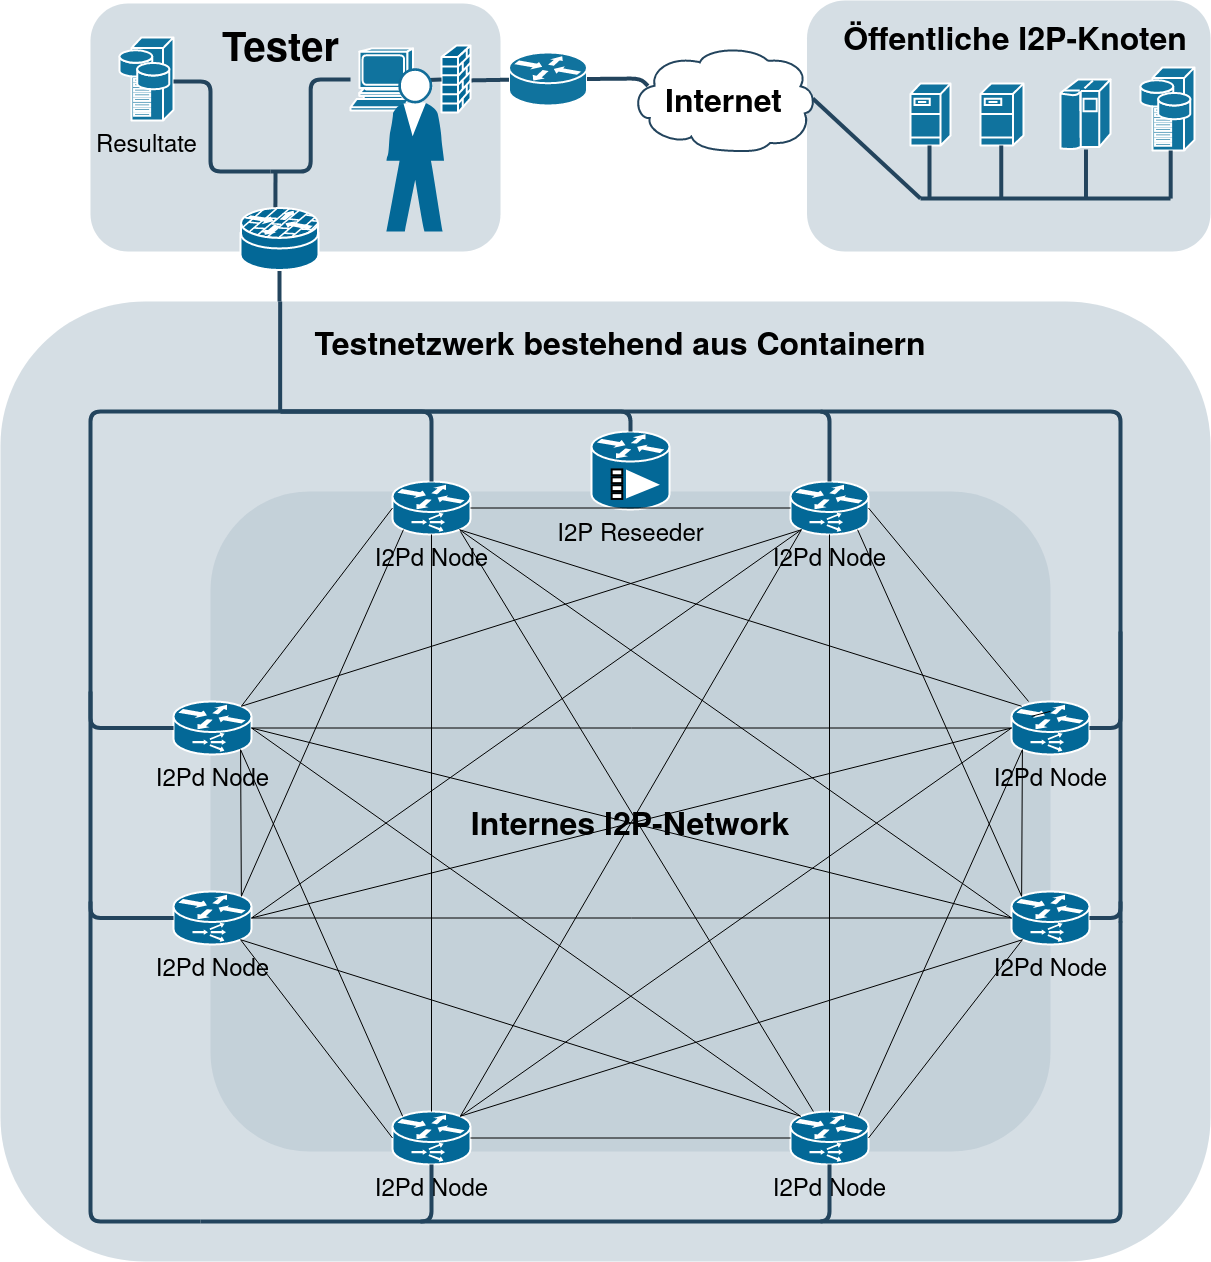
\includegraphics[width=1.0\textwidth]{i2p-testnetwork.png}
  \caption{I2P Testnetwork}\label{fig:i2p-testnetwork}
\end{figure*}

Bei der Firewall handelt es sich entweder um das Hostsystem (VM-Network) oder um das Testnetzwerk selber, welche die I2P-Knoten hostet.
Wichtig ist das der Tester, welcher das Netzwerk erstellt und die Tests durchführt sich auch ausserhalb des Testnetzwerkes befindet, um ungewollte Einflüsse zu vermeiden.
Die I2P-Knoten sind als Router dargestellt und befinden sich eigentlich alle in zwei Netzwerken gleichzeitig. Das normale IP Netzwerk und das I2P-Netzwerk.
Am Ende des Tests müssen die Testresultate an einem sicheren Ort ausserhalb des Testnetzwerks abgelegt werden, damit diese später analysiert werden können.

In der \lstinline|i2pd|-Konfiguration gibt es zusätzlich das \lstinline|familiy|-Tag, welches die Knoten als zusammenhängend markieren würde, würden diese aus Versehen mit dem echten I2P-Netzwerk reden. Dies ist auch interessant bezüglich Tests die am echten Netzwerk durchgeführt werden sollen.

%TODO: fullmesh?

\section{Bootstrapping}

Wie im Abschnitt~\fullref{sec:bootstrapping} erklärt wird im privaten Testnetzwerk ein Bootstapping-Vorgang benötigt.
Ganz zu Beginn, wenn ein Knoten dem I2P Netzwerk beitritt muss dieser wissen wo mindestens ein anderer Knoten ist.
Um dies zu bewerkstelligen wird ein separater Container dem Testnetzwerk hinzugefügt der einen Reseed-Server mit sich bringt.
Somit kann zu Beginn jeder Knoten eine Liste von anderen Knoten abfragen und so dem Netzwerk beitreten.
Anhand dieser Liste kann auch der Verbindungsgrad der Knoten gesteuert werden.
Man kann auch einen Floodfill-Router verwenden, um das Netzwerk zu bootstrappen \parencite{noauthor_bootstrapping_nodate}.
Jedoch scheint der Ansatz mit einem Reseed-Server schöner zu sein, da sich somit nicht extra Knoten im Netzwerk befindet, der die Messung beeinflussen könnte.

\section{Messen der Ressourcenauslastung}\label{sec:ressourcenauslastung}

%TODO: in kapitel latenz

Die Messung der Ressourcenauslastung der Knoten könnte aus mehreren Gründen sinnvoll sein.
Gerät ein Knoten oder die Hostsysteme für das Testnetzwerk in Ressourcenengpässe, beeinflusst dies auch die Resultate.
Dies ist insbesondere wichtig enorm wichtig bei Latenzmessungen, denn diese werden somit fehlerhaft und nicht reproduzierbar \seereq{TREP}.
Auch kann sichergestellt werden, dass das Testnetzwerk nicht so gross skaliert wurde, bzw. wie weit es skaliert werden kann \seereq{TSCL}.
Zudem kann die Test-Performance so gemessen werden \seereq{TPER}.
Folgendes könnte gemessen werden:

\begin{itemize}
    \item CPU Gebrauch (in Prozent)
    \item Netzwerkbandbreite (kbits/sec)
    \item RAM Verwendung (in Prozent)
    \item Disk I/O (read/write, kbits/sec)
    \item Freier Speicherplatz
\end{itemize}

Es wird erwartet, dass der Workload von I2P vor allem Netzwerklastig (weiterleiten über mehrere Knoten) und Prozessorlastig (Verschlüsselung) ist.
Da es sich hier um ein virtuelles Container-Netzwerk handelt, heisst dass die Last auf dem Netzwerk sich auch in der Prozessorlast zeigen wird.
Um die benötigte Anzahl Container zu starten und die I2P-Knoten zu betreiben wird auch viel Arbeitsspeicher benötigt.
